

\tikzset{every picture/.style={line width=0.75pt}} %set default line width to 0.75pt        

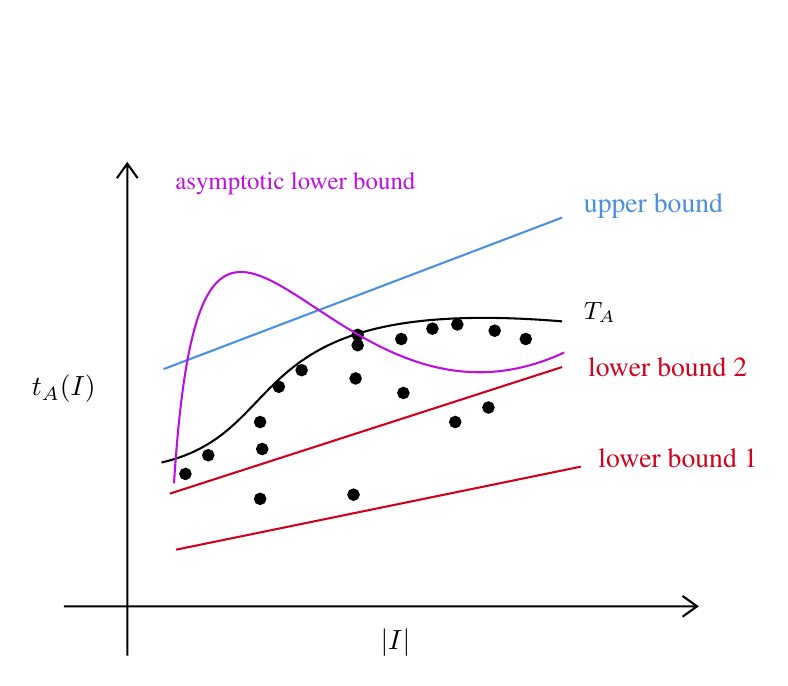
\begin{tikzpicture}[x=0.75pt,y=0.75pt,yscale=-1,xscale=1]
%uncomment if require: \path (0,300); %set diagram left start at 0, and has height of 300

%Shape: Axis 2D [id:dp46864992926435445] 
\draw  (52,232.3) -- (357,232.3)(82.5,19) -- (82.5,256) (350,227.3) -- (357,232.3) -- (350,237.3) (77.5,26) -- (82.5,19) -- (87.5,26)  ;
%Curve Lines [id:da5021464986675876] 
\draw [line width=0.75]    (99,163) .. controls (164,148) and (134,82) .. (292,95) ;
%Straight Lines [id:da36133541435794014] 
\draw [color={rgb, 255:red, 74; green, 144; blue, 226 }  ,draw opacity=1 ][line width=0.75]    (100,118) -- (292,45) ;
%Straight Lines [id:da0728433166304221] 
\draw [color={rgb, 255:red, 208; green, 2; blue, 27 }  ,draw opacity=1 ][line width=0.75]    (103,178) -- (292,117) ;
%Straight Lines [id:da6767296112625558] 
\draw [color={rgb, 255:red, 208; green, 2; blue, 27 }  ,draw opacity=1 ][line width=0.75]    (106,205) -- (301,165) ;
%Shape: Circle [id:dp42546975000741627] 
\draw  [fill={rgb, 255:red, 0; green, 0; blue, 0 }  ,fill opacity=1 ] (119,159.5) .. controls (119,158.12) and (120.12,157) .. (121.5,157) .. controls (122.88,157) and (124,158.12) .. (124,159.5) .. controls (124,160.88) and (122.88,162) .. (121.5,162) .. controls (120.12,162) and (119,160.88) .. (119,159.5) -- cycle ;
%Shape: Circle [id:dp8076707781379495] 
\draw  [fill={rgb, 255:red, 0; green, 0; blue, 0 }  ,fill opacity=1 ] (191,101.5) .. controls (191,100.12) and (192.12,99) .. (193.5,99) .. controls (194.88,99) and (196,100.12) .. (196,101.5) .. controls (196,102.88) and (194.88,104) .. (193.5,104) .. controls (192.12,104) and (191,102.88) .. (191,101.5) -- cycle ;
%Shape: Circle [id:dp17147219962617655] 
\draw  [fill={rgb, 255:red, 0; green, 0; blue, 0 }  ,fill opacity=1 ] (144,143.5) .. controls (144,142.12) and (145.12,141) .. (146.5,141) .. controls (147.88,141) and (149,142.12) .. (149,143.5) .. controls (149,144.88) and (147.88,146) .. (146.5,146) .. controls (145.12,146) and (144,144.88) .. (144,143.5) -- cycle ;
%Shape: Circle [id:dp9327712375258363] 
\draw  [fill={rgb, 255:red, 0; green, 0; blue, 0 }  ,fill opacity=1 ] (145,156.5) .. controls (145,155.12) and (146.12,154) .. (147.5,154) .. controls (148.88,154) and (150,155.12) .. (150,156.5) .. controls (150,157.88) and (148.88,159) .. (147.5,159) .. controls (146.12,159) and (145,157.88) .. (145,156.5) -- cycle ;
%Shape: Circle [id:dp48401418137987284] 
\draw  [fill={rgb, 255:red, 0; green, 0; blue, 0 }  ,fill opacity=1 ] (164,118.5) .. controls (164,117.12) and (165.12,116) .. (166.5,116) .. controls (167.88,116) and (169,117.12) .. (169,118.5) .. controls (169,119.88) and (167.88,121) .. (166.5,121) .. controls (165.12,121) and (164,119.88) .. (164,118.5) -- cycle ;
%Shape: Circle [id:dp7215414788547623] 
\draw  [fill={rgb, 255:red, 0; green, 0; blue, 0 }  ,fill opacity=1 ] (190,122.5) .. controls (190,121.12) and (191.12,120) .. (192.5,120) .. controls (193.88,120) and (195,121.12) .. (195,122.5) .. controls (195,123.88) and (193.88,125) .. (192.5,125) .. controls (191.12,125) and (190,123.88) .. (190,122.5) -- cycle ;
%Shape: Circle [id:dp47882468155096314] 
\draw  [fill={rgb, 255:red, 0; green, 0; blue, 0 }  ,fill opacity=1 ] (191,106.5) .. controls (191,105.12) and (192.12,104) .. (193.5,104) .. controls (194.88,104) and (196,105.12) .. (196,106.5) .. controls (196,107.88) and (194.88,109) .. (193.5,109) .. controls (192.12,109) and (191,107.88) .. (191,106.5) -- cycle ;
%Shape: Circle [id:dp19723118480444324] 
\draw  [fill={rgb, 255:red, 0; green, 0; blue, 0 }  ,fill opacity=1 ] (238,143.5) .. controls (238,142.12) and (239.12,141) .. (240.5,141) .. controls (241.88,141) and (243,142.12) .. (243,143.5) .. controls (243,144.88) and (241.88,146) .. (240.5,146) .. controls (239.12,146) and (238,144.88) .. (238,143.5) -- cycle ;
%Shape: Circle [id:dp06137296140295101] 
\draw  [fill={rgb, 255:red, 0; green, 0; blue, 0 }  ,fill opacity=1 ] (227,98.5) .. controls (227,97.12) and (228.12,96) .. (229.5,96) .. controls (230.88,96) and (232,97.12) .. (232,98.5) .. controls (232,99.88) and (230.88,101) .. (229.5,101) .. controls (228.12,101) and (227,99.88) .. (227,98.5) -- cycle ;
%Shape: Circle [id:dp9372562234067201] 
\draw  [fill={rgb, 255:red, 0; green, 0; blue, 0 }  ,fill opacity=1 ] (257,99.5) .. controls (257,98.12) and (258.12,97) .. (259.5,97) .. controls (260.88,97) and (262,98.12) .. (262,99.5) .. controls (262,100.88) and (260.88,102) .. (259.5,102) .. controls (258.12,102) and (257,100.88) .. (257,99.5) -- cycle ;
%Shape: Circle [id:dp6928203923385057] 
\draw  [fill={rgb, 255:red, 0; green, 0; blue, 0 }  ,fill opacity=1 ] (153,126.5) .. controls (153,125.12) and (154.12,124) .. (155.5,124) .. controls (156.88,124) and (158,125.12) .. (158,126.5) .. controls (158,127.88) and (156.88,129) .. (155.5,129) .. controls (154.12,129) and (153,127.88) .. (153,126.5) -- cycle ;
%Shape: Circle [id:dp6888865700886981] 
\draw  [fill={rgb, 255:red, 0; green, 0; blue, 0 }  ,fill opacity=1 ] (108,168.5) .. controls (108,167.12) and (109.12,166) .. (110.5,166) .. controls (111.88,166) and (113,167.12) .. (113,168.5) .. controls (113,169.88) and (111.88,171) .. (110.5,171) .. controls (109.12,171) and (108,169.88) .. (108,168.5) -- cycle ;
%Shape: Circle [id:dp7766613066440398] 
\draw  [fill={rgb, 255:red, 0; green, 0; blue, 0 }  ,fill opacity=1 ] (272,103.5) .. controls (272,102.12) and (273.12,101) .. (274.5,101) .. controls (275.88,101) and (277,102.12) .. (277,103.5) .. controls (277,104.88) and (275.88,106) .. (274.5,106) .. controls (273.12,106) and (272,104.88) .. (272,103.5) -- cycle ;
%Curve Lines [id:da14337298531359344] 
\draw [color={rgb, 255:red, 189; green, 16; blue, 224 }  ,draw opacity=1 ]   (105,173) .. controls (119,-46) and (175,165) .. (293,110) ;
%Shape: Circle [id:dp31574731151290725] 
\draw  [fill={rgb, 255:red, 0; green, 0; blue, 0 }  ,fill opacity=1 ] (254,136.5) .. controls (254,135.12) and (255.12,134) .. (256.5,134) .. controls (257.88,134) and (259,135.12) .. (259,136.5) .. controls (259,137.88) and (257.88,139) .. (256.5,139) .. controls (255.12,139) and (254,137.88) .. (254,136.5) -- cycle ;
%Shape: Circle [id:dp13435328774965294] 
\draw  [fill={rgb, 255:red, 0; green, 0; blue, 0 }  ,fill opacity=1 ] (144,180.5) .. controls (144,179.12) and (145.12,178) .. (146.5,178) .. controls (147.88,178) and (149,179.12) .. (149,180.5) .. controls (149,181.88) and (147.88,183) .. (146.5,183) .. controls (145.12,183) and (144,181.88) .. (144,180.5) -- cycle ;
%Shape: Circle [id:dp27574374905467636] 
\draw  [fill={rgb, 255:red, 0; green, 0; blue, 0 }  ,fill opacity=1 ] (239,96.5) .. controls (239,95.12) and (240.12,94) .. (241.5,94) .. controls (242.88,94) and (244,95.12) .. (244,96.5) .. controls (244,97.88) and (242.88,99) .. (241.5,99) .. controls (240.12,99) and (239,97.88) .. (239,96.5) -- cycle ;
%Shape: Circle [id:dp6960879957907262] 
\draw  [fill={rgb, 255:red, 0; green, 0; blue, 0 }  ,fill opacity=1 ] (212,103.5) .. controls (212,102.12) and (213.12,101) .. (214.5,101) .. controls (215.88,101) and (217,102.12) .. (217,103.5) .. controls (217,104.88) and (215.88,106) .. (214.5,106) .. controls (213.12,106) and (212,104.88) .. (212,103.5) -- cycle ;
%Shape: Circle [id:dp8054826566241211] 
\draw  [fill={rgb, 255:red, 0; green, 0; blue, 0 }  ,fill opacity=1 ] (213,129.5) .. controls (213,128.12) and (214.12,127) .. (215.5,127) .. controls (216.88,127) and (218,128.12) .. (218,129.5) .. controls (218,130.88) and (216.88,132) .. (215.5,132) .. controls (214.12,132) and (213,130.88) .. (213,129.5) -- cycle ;
%Shape: Circle [id:dp6729286931727385] 
\draw  [fill={rgb, 255:red, 0; green, 0; blue, 0 }  ,fill opacity=1 ] (189,178.5) .. controls (189,177.12) and (190.12,176) .. (191.5,176) .. controls (192.88,176) and (194,177.12) .. (194,178.5) .. controls (194,179.88) and (192.88,181) .. (191.5,181) .. controls (190.12,181) and (189,179.88) .. (189,178.5) -- cycle ;

% Text Node
\draw (203,241.4) node [anchor=north west][inner sep=0.75pt]    {$| I|$};
% Text Node
\draw (35,119.4) node [anchor=north west][inner sep=0.75pt]    {$t_{A}( I)$};
% Text Node
\draw (301,32) node [anchor=north west][inner sep=0.75pt]  [color={rgb, 255:red, 74; green, 144; blue, 226 }  ,opacity=1 ] [align=left] {{\fontfamily{ptm}\selectfont upper bound}};
% Text Node
\draw (303,111) node [anchor=north west][inner sep=0.75pt]  [color={rgb, 255:red, 74; green, 144; blue, 226 }  ,opacity=1 ] [align=left] {{\fontfamily{ptm}\selectfont \textcolor[rgb]{0.82,0.01,0.11}{lower bound 2}}};
% Text Node
\draw (308,155) node [anchor=north west][inner sep=0.75pt]  [color={rgb, 255:red, 74; green, 144; blue, 226 }  ,opacity=1 ] [align=left] {{\fontfamily{ptm}\selectfont \textcolor[rgb]{0.82,0.01,0.11}{lower bound 1}}};
% Text Node
\draw (301,84.4) node [anchor=north west][inner sep=0.75pt]  [font=\small]  {$T_{A}$};
% Text Node
\draw (101,22) node [anchor=north west][inner sep=0.75pt]  [font=\small,color={rgb, 255:red, 189; green, 16; blue, 224 }  ,opacity=1 ] [align=left] {\begin{minipage}[lt]{91.44912000000001pt}\setlength\topsep{0pt}
\begin{center}
{\fontfamily{ptm}\selectfont asymptotic lower bound}
\end{center}

\end{minipage}};


\end{tikzpicture}